\section{Architecture}
\label{sec:architecture}
StocNoC follows mesh topology with each processing element (PE) along with its network interface (NI) representing a \emph{node} in the contact network.
Nodes are interconnected with the help of switches and bi-directional physical links as shown in~Fig.~\ref{figure:noc}.
The NoC configuration and inter-node communication are supported via packet switching.
The bottom left switch acts as the communication interface with external world, through which configuration packets are sent as well as the network status is monitored.
An external host such as a server computer configures the NoC for the target network and monitors the network status as time progresses. 
By analyzing the packets received from the network, the host can determine the specific nodes that are infected, nodes that have recovered, and the overall spreading pattern of the process.



\subsection{Packet Formats}
StocNoC manages configuration as well as inter-node communication using the different packet formats shown in Fig.~\ref{figure:pktformat}.
It supports unicast, multicast and broadcast packet transmissions based on the packet~\emph{type}. 
Unicast packets are used for node configuration~(at zero epoch or at $t = 0$) by an external host. 
The target node address (X and Y coordinates of the node) is stored in the \emph{destination address} field and the configuration data are carried in the \emph{input number (in)} and \emph{initial status (is)} fields. 
The \emph{input number} configures the number of neighbors (number of nodes connected to this node based on the adjacency matrix) and the \emph{initial status} configures whether the node is infected or susceptible at zero epoch.

Multicast packets are used for inter-node communication, where each node updates all its neighbors with its status after each epoch (each discrete time in simulation).
Rather than sending the same packet to each of its neighbors, each node injects a single packet to the NoC and the unique router design duplicates the packets close to the target nodes.
This considerably reduces the network routing congestion and improves the overall latency.
The packet carries the address of the injecting node in the \emph{source address} field and the status (infected/susceptible) in the \emph{status (s)} field.
Due to the packet switched nature of the NoC, it is possible that packets are delivered out-of-order to the destination nodes.
To manage this, each multicast packet carries a \emph{sequence number (sn)} field, which specifies the discrete simulation time.
Every packet in the network originating at the same discrete simulation time will have the same sequence number.

Since all nodes in the network share the same infection~($\beta$) and recovery rates~($\gamma$), this information is broadcasted across the network at the beginning of the simulation. 
Again, the router design and the routing algorithm enables injecting a single packet from the external host and the packet being replicated and delivered to each node.
The \emph{rate segment} of the packet initializes a portion of the pseudo random binary sequence (PRBS) generator used in the network interface discussed in Section~\ref{sec:ni}.
Since the current implementation uses a 100-bit long PRBS and the rate segment is only 10-bits wide, 10 configuration packets are required to initialize them. 
NoC configuration packets are special broadcast packets that configure the routing tables~(RTs) inside the switches. 
Each packet configures a portion of an RT and multiple packets are required to configure the entire network.
\begin{figure}[t!]
	\begin{center}
    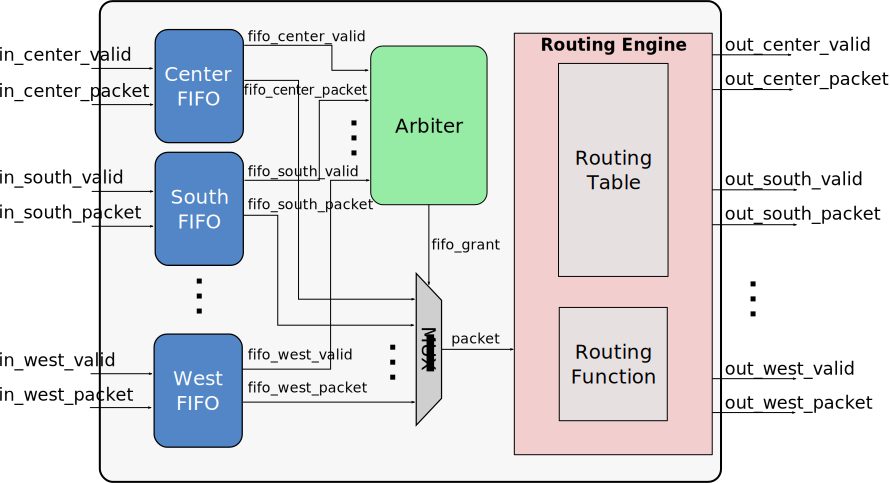
\includegraphics[width=0.8\columnwidth]{Figures/ROUTER.pdf}
    \caption{The NoC switch architecture with store-and-forward functionality and support for unicast and multicast routing.} 
    \label{figure:router}
    \end{center}
    \vspace{-5mm}
\end{figure}

\subsection{Switch}
The overall architecture of the StocNoC switch is depicted in Fig.~\ref{figure:router}.
The switch follows store and forward architecture with each interface (from 4 neighboring switches and the node) connected to an input FIFO.
Every switch interface follows AXI4-Stream protocol~\cite{xilinxaxi}.
To limit resource utilization, output FIFOs are omitted in the design.
An arbiter chooses one of the input FIFOs for packet transmission based on their requests following a round-robin scheme.
This avoids resource starvation and minimizes packet queueing delays. 
The \emph{fifo\_grant} signal from the arbiter drives the output of a multiplexer which selects the appropriate FIFO output for packet transmission. 

The selected packet is forwarded to the routing engine~(RE).
The RE logic first checks for the packet type.
Unicast packet~(PE configuration packets) routing is managed by a routing function (RF) and multicast packet~(PE status packets) routing is managed by a routing table~(RT).
The RF logic implements the traditional dimension-ordered XY routing by comparing the destination address embedded in the packet with the switch's address~\cite{Chawade2012}.

Multicast routing scheme is deployed for status packets to reduce the network congestion and latency.
This method also frees nodes from storing the RTs thus, making their design relatively simple.
A node sending its status puts only its source address into the packet and injects to the corresponding switch, unaware of the packet's ultimate targets.
Each entry in the RT used for multicast routing is 5 bits wide and the RT depth is same as the overall network size~(number of nodes in the network).

The source address embedded in the multicast packets serves as the RT entry number.
Each bit in a table entry determines the directions in which a packet originating from the corresponding address will be forwarded.
The broadcast could be to one or more of the neighboring switches as well as the to the node interfaced with the switch.
By appropriately configuring the RTs, packets from any node can be broadcasted to any given subset of nodes within the network. 
The routing path taken by each packet is similar to \emph{tree routing}, where the root of a tree is the source node and the destination nodes are located at the tree branches and leaves. 
If the destination nodes are located along the tree branches, intermediate switches perform forward-and-absorb operation. 
Traditional tree routing suffers from the possibility of deadlocks~\cite{Samman2010} in the intermediate nodes, but combining it with XY routing circumvents this possibility. 

\begin{figure}[t!]
    \begin{center}
    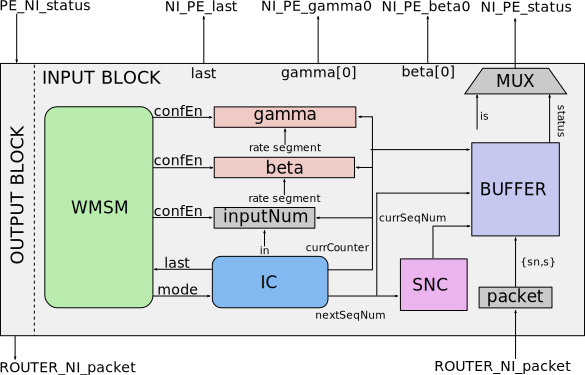
\includegraphics[width=0.8\columnwidth]{Figures/NI.pdf}
    \caption{Network Interface Architecture.} 
    \label{figure:ni}
    \vspace{-5mm}
    \end{center}
\end{figure}

The content of each RT is determined offline by an application based on the network adjacency matrix. 
For a network with \emph{NETWORK\_SIZE} nodes, aspect ratios \emph{X} and \emph{Y}, and adjacency matrix \emph{adjacencyMatrix[NETWORK\_SIZE]$\\*$[NETWORK\_SIZE]}, each table entry \emph{i} corresponding to each switch \emph{j} is generated based on Algorithm~\ref{algo}. 
The entire RT is injected to the network through the bottom-left switch as NoC configuration broadcast packets.
This approach is taken to keep packets sizes small, as packets do not carry information regarding router and RT address. 
From the received broadcast packets, each switch selects only the portions corresponding to its RT and transmits the entire table to the neighboring switch to its right.
Switches along the first column of the NoC transmits these packets to the neighboring switches in the north direction as well.
The switch's knowledge about its own address and an internal packet counter enables this configuration strategy.
Each packet carries only a fraction of the table (10-bits or 2 entries) and may require thousands of packets for complete configuration.
\begin{algorithm}[!t]
	\caption{Routing Table Generation}
	\begin{algorithmic}[1]
		\State Clear all RT entries.
		\For{j =0; j$\textless$NETWORK\_SIZE; j=j+1}
     		\For{i =0; i$\textless$NETWORK\_SIZE; i=i+1}
         		\If{adjacencyMatrix[j][i]==1}
             		\State inAddr=i;
             		\State outAddr=j;
             		\State RT[i][j][CENTER] = 1;
            		\If{outAddr [X]$\textgreater$ inAddr [X]}
                		\For{x=outAddr[X]; x$\textgreater$inAddr[X];x=x-1}
                    		\State RT[outAddr[Y]$\times$XSIZE+x][j][WEST]=1
                		\EndFor
             		\Else
                		\For{x=outAddr[X];x$\textless$inAddr[X];x=x+1}
                    		\State RT[outAddr[Y]$\times$XSIZE+x][j][EAST]=1
                		\EndFor
            		\EndIf
             		\If{outAddr[Y]$\textgreater$inAddr[Y]}
                		\For{y=outAddr[Y];y$\textgreater$inAddr[Y];y=y-1}
                   			\State RT[y$\times$XSIZE+inAddr[X]][j][SOUTH]=1
                		\EndFor
             		\Else
             			\For{y=outAddr[Y];y$\textless$inAddr[Y];y=y+1}
                    		\State RT[y$\times$XSIZE+inAddr[X]][j][NORTH]=1
                		\EndFor
             		\EndIf
         		\EndIf
     		\EndFor
 		\EndFor
\end{algorithmic}
\label{algo}
\end{algorithm}
\setlength{\textfloatsep}{15pt}

\subsection{Network Interface (NI)}
\label{sec:ni}

The NI module manages the communication between a switch and the corresponding PE. Moreover, it also implements the logic to control the state of the node after each discrete simulation time.
Its detailed architecture is depicted in Fig.~\ref{figure:ni}.
The \emph{working mode state machine} (WMSM) manages the operating mode of a node, which may be either in \emph{configuration state} or in \emph{running state}.
When the network is in the configuration state, WMSM routes the configuration packets received from the switch interface to appropriate destination registers.
The contents of the unicast packet specifying the number of neighbors of the node is stored in the \emph{inputNum} register.

The discrete time probabilities required to decide the state of a node (whether infected or susceptible) are implemented by the \emph{gamma} and \emph{beta} PRBS generators.
Both are linear feedback shift registers (LFSRs) composed of $100$ flip-flops with the last stage feeding back to the first stage.
In order to implement a specific rate (infection or recovery), the corresponding probability is multiplied by $100$ and the LFSR is initialized with a random binary pattern with number of ones equal to the result of multiplication. 
For example, to achieve a $\beta$ value of $0.3$, the $100$ flip-flops in the \emph{beta} LFSR are initialized with a random binary pattern with $30$ ones and $70$ zeros.
The initialization values for the two PRBS generators are received as broadcast packets from the external host.
Since the size of PRBS generators is much larger than the packet size, multiple configuration packets are required to initialize them.
The \emph{Input Counter (IC)} logic specifies the index number of the PRBS generators to which the incoming configuration packet values are written.
%The WMSM routes the initialization data to the appropriate PRBS based on the status signals from IC.


After initialization, the LSFRs freely run and the least significant bit (LSB) is used for achieving the required rate.
Due to the initialization pattern, the probability of the LSB becoming one will be same as the required rate.
This is similar to finding a number between $0$ and $1$ from a uniform distribution and checking whether its value is less than the required rate.
This software approach is emulated in hardware through the said mechanism.
The initialization patterns are generated offline through a software application and broadcasted to the nodes through multiple packets as discussed before.
Although same initialization packets are broadcasted to all the nodes, due to the inherent latency in packet switching, each LFSR will have a different initialization pattern at epoch zero but representing the same rate.

Once the WMSM receives the unicast packet carrying the initial node status, it is transferred to the PE and is switched to \emph{running state}. 
When a PE receives its initial status, it is immediately broadcasted to its neighbors.
Thus,some PEs may possibly receive packets from its neighbors before the end of the configuration. 
Moreover, due to path length differences and different congestion levels along different paths, out-of-order packets may arrive even at running state which may result in a node receiving a status from one of its neighbors for the next discrete time before receiving all status for the current time. 


\begin{figure}[t!]
    \begin{center}
    
\includegraphics[width=0.7\columnwidth]{Figures/ISSM.pdf}
    \caption{SIS State machine} 
    \label{figure:fsm}
    \end{center}
    \vspace{-5mm}
\end{figure}

To overcome the out-of-order status delivery, PEs embed a sequence number into the status packets.
The sequence number indirectly represents the current discrete time.
When status packets are received, they are initially stored in a buffer with logical partition for each sequence number.
Each partition can store NETWORK\_SIZE number of status and each entry is just one $1$ bit wide (to represent infected or susceptible).  
Each partition maintains its own counter which counts the number of status that have already arrived and to which entry the next status will be updated. 
In running mode, the status are extracted from a partition specified by the \emph{sequence number checker} (SNC) one at a time and transferred to the PE.
The status are sent to the PE only after receiving the status from all its neighbors, whose number is specified in the \emph{inputNum} register during configuration.
Once all status are sent, the SNC is incremented to select the next partition.
Since each PE generates a status packet only after receiving the status from all its neighbors, it could be proven that two sequence numbers are enough to distinguish between different discrete times. 
Thus, the size of the buffer is $2 \times $NETWORK\_SIZE bits to support two partitions.

\subsection{Processing Element (PE)}

Each PE runs the SIS state-machine, similar to the one shown in Fig.~\ref{figure:fsm}.
The initial infection status is received from the NI during the configuration stage.
Once the NI receives status from all the neighbors for a discrete time, it transfers the status one at a time to the PE.
If the PE is in susceptible state and receives an infected status from one of the neighbors, it checks the output of the \emph{beta} PRBS generator.
If the PRBS output is high, the PE state is switched to \emph{infected}.
Further status received from the neighbors are ignored for the current epoch since, in the SIS model, a node cannot change its state more than once in any discrete time. 
If the PE is in \emph{infected} state, it checks the output from \emph{gamma} PRBS generator after receiving status from all neighbors.
If the PRBS output is high, the state is switched to \emph{susceptible} and the status of the neighbors play no role in this state transition.
In all cases, the status of the PE after a discrete time is sent to the NI module which is then multicasted to all its neighbors.

The SIS state-machine is relatively simple, but due to the modular design approach any other model can be easily incorporated by modifying this state-machine alone.
In future, as cloud FPGA instances start supporting partial reconfiguration (PR), models can be dynamically updated by only reconfiguring the PE module which substantially reduces the design and configuration time.



\subsection{Simulation Steps}
The host computer executes the following steps for StocNoC-based SIS model simulation:
\begin{itemize}
	\item Inject the NoC configuration broadcast packets to configure the routing tables (\figurename{~\ref{figure:pktformat}d}).
\item Inject the broadcast packets to configure $\beta$ and $\gamma$ (\figurename{~\ref{figure:pktformat}c}).
\item Inject the unicast packets to configure the number of neighbors to each node (\figurename{~\ref{figure:pktformat}a}).
\item Inject the unicast packets to configure the initial status of each node (\figurename{~\ref{figure:pktformat}a}).
\item Receive packets from the NoC and monitor the network status. Once status packets are received from all nodes, increment the discrete time step and log the number of infected and susceptible nodes.
\end{itemize}